\documentclass[12pt]{article}
\usepackage{amsmath}
\usepackage{times}
\usepackage{graphicx}
\usepackage{color}
\usepackage{multirow}
\usepackage{mathptmx} % Times-like text + math
\usepackage[T1]{fontenc}
\usepackage{hyperref}
\usepackage{makecell}
\usepackage{booktabs}
\usepackage{tabularx}
\usepackage{amsmath, amssymb}
\usepackage{array}

%%%
\usepackage{tabularx,booktabs}
\usepackage{ragged2e}
\newcolumntype{Y}{>{\RaggedRight\arraybackslash}X}

\usepackage{natbib}
\bibliographystyle{apalike}


\usepackage{setspace}
\setstretch{1.05}

\usepackage{microtype}
\setlength{\emergencystretch}{2em}

\usepackage{graphicx}
%\usepackage[authoryear]{natbib}
%
\usepackage{bbm}
\usepackage{latexsym}
%\DeclareGraphicsExtensions{.eps,.png}

%%% margins 
\textheight 23.4cm
\textwidth 14.65cm
\oddsidemargin 0.375in
\evensidemargin 0.375in
\topmargin  -0.55in
%
\renewcommand{\baselinestretch}{1.05}
%
\interfootnotelinepenalty=10000
%
\renewcommand{\thesubsubsection}{\arabic{section}.\arabic{subsubsection}}
\newcommand{\myparagraph}[1]{\ \\{\em #1}.\ \ }
\newcommand{\citealtt}[1]{\citeauthor{#1},\citeyear{#1}}
\newcommand{\myycite}[1]{\citep{#1}}

% Different font in captions
\newcommand{\captionfonts}{\normalsize}

\makeatletter  
\long\def\@makecaption#1#2{%
  \vskip\abovecaptionskip
  \sbox\@tempboxa{{\captionfonts #1: #2}}%
  \ifdim \wd\@tempboxa >\hsize
    {\captionfonts #1: #2\par}
  \else
    \hbox to\hsize{\hfil\box\@tempboxa\hfil}%
  \fi
  \vskip\belowcaptionskip}
\makeatother   
%%%%%

\renewcommand{\thefootnote}{\normalsize \arabic{footnote}} 	

\begin{document}
\hspace{13.9cm}1

\ \vspace{20mm}\\

\begin{center}{\LARGE Event-Time Distribution Modeling for Robust EEG-Based Reaction-Time Prediction}
\end{center}

\ \\
{\bf \large Ayana Mussabayeva$^{1}$\textsuperscript{*}}\\
ayana.mussabayeva@mbzuai.ac.ae

\ \\ {\bf \large Anuar Aimoldin$^{1}$\textsuperscript{*}}\\
anuar.aimoldin@mbzuai.ac.ae

% \ \\
% {\bf \large Ayana Mussabayeva$^{\displaystyle 1}$}\\
% ayana.mussabayeva@mbzuai.ac.ae


% \ \\ {\bf \large Anuar Aimoldin$^{\displaystyle 1}$}\\
% anuar.aimoldin@mbzuai.ac.ae

\ \\ {\bf \large Yedige Mussabayev$^{\displaystyle 2}$}\\
ymussabayev@hof-university.de

\ \\ {\bf \large Xue Liu$^{\displaystyle 1, 3}$}\\
steve.liu@mbzuai.ac.ae

\ \\ {\bf \large Kun Zhang$^{\displaystyle 1, 4}$}\\
kun.zhang@mbzuai.ac.ae


\ \\
{$^{\displaystyle 1}$Mohamed bin Zayed University of Artificial Intelligence (MBZUAI), Abu Dhabi, UAE}
\ \\
{$^{\displaystyle 2}$ Hof University, Hof, Germany}
\ \\
{$^{\displaystyle 3}$ McGill University, Montreal, QC, Canada}
\ \\
{$^{\displaystyle 4}$ Carnegie Mellon University, Pittsburgh, PA, USA}
\ \\
{\normalsize \textsuperscript{*}Equal contribution}\\




\ \\[-2mm]
{\bf Keywords:} robust EEG decoding, event-time distribution modeling, behavioral decoding, temporal segmentation

\thispagestyle{empty}
\markboth{}{NC instructions}
%
\ \vspace{-0mm}\\
%
%Abstract
\begin{center} {\bf Abstract} \end{center}



Robust EEG decoding remains challenging due to low signal-to-noise ratio and pronounced distribution shift across
subjects, sessions, and acquisition setups. We study robust EEG decoding under cross-subject and cross-release
distribution shift on Healthy Brain Network EEG recordings from the contrast change detection paradigm. Our central idea
is that making task-relevant temporal structure explicit improves robustness under EEG heterogeneity, and we apply it to behavioral decoding (trial-wise reaction time, RT) from stimulus-locked 2~s windows.


We replace scalar regression with temporal segmentation: models predict an event-time
distribution using Gaussian-smoothed targets and distribution-matching losses, followed by a soft-argmax readout and
out-of-fold stacking over distributional meta-features.
This framing is useful for brain-behavior decoding when targets are inherently temporal. It aligns supervision with latency variability, enables latent-consistent jittered cropping, and provides an uncertainty signal for more robust ensembling under cross-subject or session shift. We also report competitive lightweight regression baselines under the same subject-disjoint protocol as reference points for ablations. In our experiments, improvements were more sensitive to objective design and distribution-aware ensembling than to moderate increases in model capacity within the tested regime.









\section{Introduction}
Electroencephalography (EEG) is one of the most widely used techniques for measuring human brain activity, largely because it is noninvasive, comparatively inexpensive, and offers millisecond-scale temporal resolution. These properties make EEG a natural sensing modality for closed-loop and interactive systems, including brain--computer interfaces (BCIs), where decisions must be made real-time based on ongoing neural dynamics.
EEG-driven BCIs have been investigated for decades, from early communication systems \citep{FarwellDonchin1988P300Speller}
to applications in neurorehabilitation \citep{Hamedi2016BCIRehabReview}, real-time neuromodulation
\citep{Zrenner2018EEGStateDependentTMS}, and interactive entertainment \citep{Lecuyer2008BCIVRVideogames}.

Motivated by the success of foundation models in language and vision, the EEG community has recently seen a rapid growth of large-scale pretrained backbones that aim to learn transferable, task-agnostic representations from heterogeneous EEG corpora. Examples include transformer-based pretraining such as EEGPT \citep{wang2024eegpt}, large multi-dataset tokenization and masking strategies such as LaBraM \citep{Jiang2024LaBraM} and EEGFormer \citep{Chen2024EEGFormer}, state-space model backbones such as EEGMamba \citep{Wang2025EEGMamba}, and large-scale cross-setup pretraining explicitly targeting montage and recording variability such as REVE \citep{ElOuahidi2025REVE}. Autoregressive pretraining has also been explored for generalist EEG modeling \citep{Yue2024BrainGPT}. Overall, these efforts suggest that large-scale self-supervised pretraining can reduce reliance on task-specific labels and improve performance.

Despite this progress, robust EEG decoding remains challenging in practice due to low signal-to-noise ratio (SNR) and strong distribution shifts. EEG recordings reflect mixtures of neural sources through volume conduction and are easily contaminated by non-neural artifacts such as eye movements, facial and neck muscle activities, cardiac signals, and environmental noise. EEG is also highly nonstationary across time and context: changes in alertness, movement, task engagement, and electrode impedance can substantially shift the data distribution even within a single session. Crucially for machine learning, there is substantial inter-subject variability driven by anatomy, development, cognitive strategy, and recording conditions. Together, these factors often yield models that perform well within-subject or within-session but degrade sharply when evaluated across subjects, sites, or dataset releases.

In this work, we argue that a practical route to robustness under such heterogeneity is to make temporal structure explicit, rather than treating each example as a static input-output regression problem.
We study two complementary settings where supervision is weak and SNR is low, and where temporal structure is naturally informative. 
First, we consider behavioral decoding: trial-wise reaction time prediction, where behavior is expressed through event timing within a stimulus-locked window. 
Second, we consider trait prediction: a stable, participant-level externalizing psychopathology factor from short segments, where the label signal is even weaker and must be captured through consistent temporal coupling patterns. 
Given the low-SNR and cross-subject/cross-release shift, we deliberately prioritize lightweight models and low-dimensional descriptors, focusing on inductive bias (explicit temporal structure) and robust combination strategies rather than scaling model size.

We evaluate these ideas using the EEG Foundation Challenge benchmark \citep{EEGFoundationChallengeArxiv2025}, which stress-tests generalization under cross-subject and cross-release shift. The benchmark is built on the Healthy Brain Network EEG dataset spanning thousands of pediatric and adolescent participants and multiple experimental paradigms \citep{Shirazi2024HBNEEG}. We focus on the Contrast Change Detection (CCD) paradigm and its two associated prediction problems: trial-wise reaction time and subject-level externalizing.

For reaction-time decoding, we reframe scalar regression as temporal segmentation: instead of predicting a single reaction-time value directly, we supervise models to produce an event-time distribution over the response window using Gaussian-smoothed targets and distribution-matching losses. This formulation supports temporally consistent augmentation, yields uncertainty signals useful for calibration and ensembling, and improves robustness under jitter and distribution shift. For externalizing prediction, we propose a complementary and interpretable lagged dynamics descriptor pipeline based on multi-lag correlations and ridge-stabilized transition operators, making temporal coupling explicit in a low-dimensional representation. Together, these methods operationalize a shared principle: explicitly modeling temporal structure, either event timing for behavior or lagged coupling for traits, can stabilize learning under low SNR and heterogeneous EEGs.

Finally, in this benchmark setting we observe that strong held-out performance can be achieved with lightweight models and lightweight descriptors. While this is not a controlled scaling analysis, it is consistent with the view that under heterogeneous EEG and cross-release shift, objective design and distribution-aware ensembling can be more influential than moderate increases in model capacity within the tested regime.

\section{Related Work}

\subsection{Robust EEG Decoding under Shift}
A central obstacle for EEG decoding is that the data distribution changes substantially across subjects, sessions, and
recording setups. Long before the current wave of large pretrained EEG backbones, the BCI community developed methods
explicitly aimed at mitigating this shift through feature spaces and normalization procedures designed to be more stable
than raw sensor-space signals. A prominent line of work represents trials by spatial covariance matrices and performs
classification using the geometry of symmetric positive definite (SPD) matrices, yielding strong cross-subject and
cross-session performance in multiple paradigms \citep{Barachant2012RiemannianBCI}. Building on this, transfer learning
work in EEG-BCIs has emphasized distribution alignment and the reuse of data across subjects/sessions to reduce or avoid
subject-specific calibration \citep{Jayaram2016TransferLearningBCI,Zanini2018RiemannianTL,HeWu2020EuclideanAlignment}.
These approaches underscore a recurring theme: robustness often benefits from inductive biases (e.g., geometry-aware
representations, explicit alignment) that reduce nuisance variability before or during learning.

More recently, deep-learning approaches to robustness have imported ideas from domain adaptation, including learning
domain-invariant representations by adversarial objectives \citep{Ganin2016DANN} or by matching second-order statistics
across domains \citep{SunSaenko2016DeepCORAL}. In EEG, these ideas are typically instantiated as subject- or session-level
alignment modules, discrepancy losses, or adversarial heads that encourage invariance to subject identity while retaining
task-relevant information. In parallel, self-supervised and large-scale pretraining has emerged as another route to transferability: contrastive or masked objectives can learn reusable representations across tasks and hardware
\citep{Kostas2021BENDR}, and this direction has expanded rapidly into multi-dataset EEG foundation models
\citep{wang2024eegpt,Jiang2024LaBraM,Chen2024EEGFormer,Wang2025EEGMamba,ElOuahidi2025REVE,Yue2024BrainGPT}.

Our work is complementary to both alignment-centric transfer learning and large-scale pretraining. Rather than proposing
a new invariant backbone or an explicit domain-matching loss, we focus on a task-driven principle: \emph{make
task-relevant temporal structure explicit}. The NeurIPS EEG Foundation Challenge defines two complementary tasks (\citep{EEGChallengeWebsite2025, EEGFoundationChallengeArxiv2025}). For Challenge~1, this means explicitly modeling \emph{when} the behavioral
event occurs within the stimulus-locked window; for Challenge~2, it means explicitly summarizing \emph{lagged coupling}
patterns that are plausibly more stable across heterogeneous recordings than instantaneous sensor values. In this sense,
we aim to obtain robustness from objective/representation design that exposes temporally meaningful structure, while
keeping the core models lightweight.

\subsection{Behavioral Decoding as Event Timing / Time-to-Event}
Reaction time (RT) and related behavioral measures are inherently temporal: even when evaluation uses a single scalar per
trial, the latent object of interest is an \emph{event time} within a post-stimulus window. Cognitive neuroscience has a
long tradition of modeling response times as distributions governed by latent decision processes (e.g., accumulation-to-bound
models), and EEG analyses often distinguish stimulus-locked from response-locked components, where response-related
dynamics can shift in latency across trials. Early work on single-trial ERP analysis and visualization emphasized this
point by sorting trials by RT and revealing response-locked structure that is blurred by averaging \citep{Jung1998SingleTrialERP}.
In parallel, supervised RT prediction from single-trial EEG has been explored using classical features or deep models,
typically treating RT as direct regression or coarse discretized classification \citep{Chowdhury2020RTSensors}.

From a machine-learning perspective, reframing scalar regression as distributional prediction has several precedents.
Label distribution learning (LDL) treats supervision as a distribution over labels rather than a single point value,
providing a natural language for ``soft'' targets and distribution-matching losses \citep{Geng2016LabelDistributionLearning}.
Time-to-event (survival) modeling similarly targets the distribution of event times, classically via hazard-based models
\citep{Cox1972CoxPH} and more recently via deep models that directly parameterize discrete-time event distributions
\citep{Lee2018DeepHit}. Although our RT setting is not survival analysis in the clinical sense (there is no censoring
mechanism in the benchmark protocol), the conceptual alignment is useful: predicting an event-time distribution makes
timing explicit, supports calibration/uncertainty analysis, and can be more compatible with temporal jitter and
cropping than point regression.

Our segmentation formulation adopts this perspective in a minimal way tailored to short EEG windows: we supervise a
probability mass function over discretized post-stimulus time bins using smoothed targets and distributional losses, then
extract RT via a differentiable readout. This bridges single-trial EEG traditions that highlight response-locked latency
variability \citep{Jung1998SingleTrialERP} with modern distributional supervision frameworks \citep{Geng2016LabelDistributionLearning,Lee2018DeepHit},
while remaining computationally lightweight.

\subsection{Trait Prediction from Temporal Coupling / Connectivity Descriptors}
Predicting stable traits or psychopathology dimensions from short, weakly labeled EEG segments is challenging because the
label signal is not tied to a specific within-window event. One influential line of work links externalizing-related
psychopathology to reliable EEG/ERP markers, especially reduced P300 amplitude and related time--frequency signatures.
A substantial literature supports P3 amplitude reduction as an endophenotype indexing risk for substance use and related
externalizing outcomes \citep{Iacono2003P300Externalizing,IaconoMalone2011P300Endophenotype,Patrick2006P300Externalizing,Hicks2007GenesP3Externalizing}.
These findings suggest that trait-relevant information can be expressed through stable dynamical properties (e.g., how
neural populations coordinate over time), not only through transient event-locked responses.

A natural way to operationalize such dynamical information is through measures of functional and directed connectivity.
Functional connectivity metrics (coherence, phase synchronization, phase-slope index, etc.) are widely used but come with
well-known interpretational pitfalls in EEG, including volume conduction, common reference effects, and sample-size bias;
tutorial reviews emphasize careful choice of metrics and controls \citep{BastosSchoffelen2015ConnectivityTutorial}. To
mitigate spurious ``zero-lag'' coupling due to mixing, measures such as imaginary coherency and phase-lag index (PLI)
down-weight instantaneous correlations that can arise from common sources \citep{Nolte2004ImaginaryCoherency,Stam2007PLI}.
For directed dependencies, autoregressive modeling and Granger-style predictability provide a statistical notion of
directed influence \citep{Granger1969,BarnettSeth2014MVGC,Seth2015GrangerNeuro}, though their assumptions and sensitivity
to preprocessing must be respected in neurophysiological settings.

Our externalizing pipeline sits in this connectivity tradition but is deliberately constrained for robustness and
interpretability under short windows and cross-release shift. Instead of estimating high-variance spectral connectivity or
full multivariate causal graphs, we summarize lagged temporal coupling using (i) multi-lag cross-correlations and (ii)
ridge-stabilized transition operators that capture predictable lag structure in a low-dimensional form. The goal is not
to claim mechanistic connectivity, but to extract coupling descriptors that are stable enough to generalize across
heterogeneous recordings and informative for subject-level traits that have known EEG correlates
\citep{Iacono2003P300Externalizing,IaconoMalone2011P300Endophenotype}.

\section{Dataset and Benchmark Tracks}

We use the NeurIPS EEG Foundation Challenge benchmark \citep{EEGChallengeWebsite2025}, based on curated releases of the HBN-EEG dataset \citep{Shirazi2024HBNEEG}, to evaluate robustness under cross-subject and cross-release distribution shift. The benchmark provides a labeled \emph{development} release and a fully hidden \emph{held-out} release, for which inference and scoring are performed server-side on the challenge platform. We consider two benchmark tracks: (i) trial-wise reaction time prediction (Challenge~1; behavioral decoding) and (ii) subject-level psychopathology factor prediction (Challenge~2; trait prediction). The releases comprise recordings from more than 3{,}000 participants aged 5--21 collected across a standardized battery of six EEG tasks spanning both passive and active paradigms \citep{Shirazi2024HBNEEG,EEGChallengeWebsite2025}.

HBN-EEG is distributed in a Brain Imaging Data Structure (BIDS)-compatible format with detailed event annotations using Hierarchical Event Descriptors (HED), enabling reproducible
preprocessing and time-locked analyses \citep{Shirazi2024HBNEEG}. In the original acquisition, EEG was recorded in a
sound-shielded environment using a high-density 128-channel EGI Geodesic HydroCel system at 500~Hz
(online 0.1--100~Hz bandpass), referenced at Cz, with electrode impedances maintained below 40~k$\Omega$.
For the challenge, the organizers provide a harmonized derivative of these recordings that is band-pass filtered
(0.5--50~Hz) and downsampled to 100~Hz to standardize modeling across releases \citep{EEGChallengeWebsite2025}.
In the released derivatives, a total of 129 channels are included (128 EEG channels plus a reference); throughout this
work we train models on the 128 EEG channels and exclude the reference channel from the learnable input.

In addition to EEG and demographics, the releases include continuous psychopathology dimensions derived from parent-reported
Child Behavior Checklist (CBCL) data via a confirmatory bifactor model: a general \emph{p}-factor alongside orthogonal
specific factors for internalizing, externalizing, and attention-hyperactivity \citep{HBN_Factsheet_EEGChallenge}.
In this work, we focus on the externalizing factor, which captures variance related to behavioral dysregulation
(e.g., rule-breaking/aggressive and conduct-like problems) \citep{HBN_Factsheet_EEGChallenge}.

One of the active paradigms in HBN-EEG and the focus of both benchmark tracks is the contrast change detection (CCD) task.
In each CCD trial, participants viewed two concentric, flickering grating stimuli (one left-tilted and one right-tilted).
After a variable delay, the contrast of one stimulus increased, making it perceptually dominant. Participants were
instructed to respond as quickly as possible to indicate whether the dominant grating was left or right-tilted, after which
they received immediate accuracy feedback (smiley for correct, sad face for incorrect). The CCD recordings support two
complementary prediction settings that emphasize different temporal structure: event-locked response timing for trial-wise
behavior and segment-level temporal coupling for subject-level traits.

\subsection{Challenge 1: Reaction Time Prediction in CCD}
The goal of Challenge~1 is behavioral decoding via prediction of the reaction time (RT) of the participant's button press
on each CCD trial. The model is provided with a fixed-length 2~s EEG segment (128 channels at 100~Hz)
time-locked to the stimulus event. In the competition's official inference setup (including the held-out release), the
2~s input window corresponds to the interval from 0.5~s to 2.5~s after stimulus onset (Figure~\ref{fig:tasks});
trials whose responses fall outside this interval are excluded by the benchmark construction.
The target is a single scalar RT per trial, and performance is evaluated using normalized RMSE (nRMSE), defined as RMSE
divided by the standard deviation of the true targets \citep{EEGChallengeWebsite2025}. Because the label reflects when a
response occurs within the post-stimulus interval, this prediction problem naturally motivates modeling RT as an event-time
quantity rather than a static scalar regression target.

\begin{figure}[!t]
    \centering
    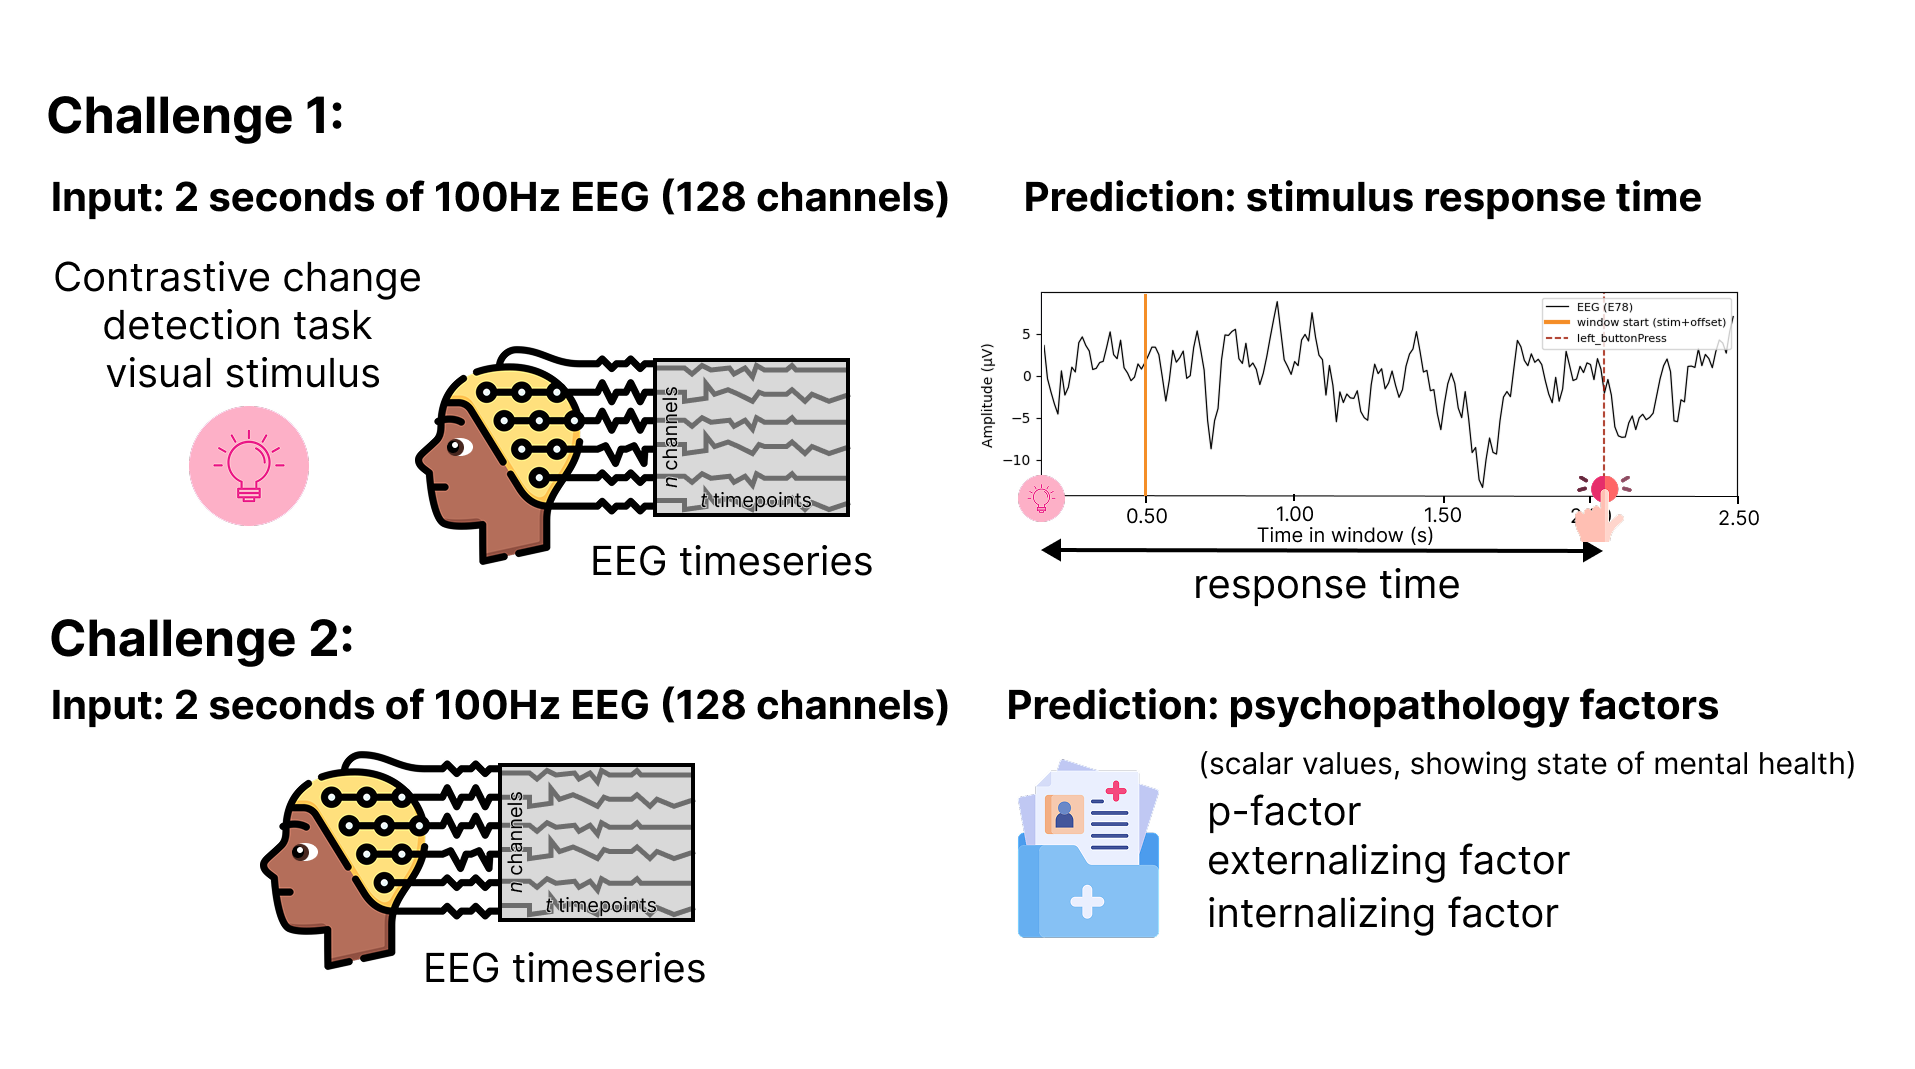
\includegraphics[width=0.9\linewidth]{img/challenge_tasks.png}
    \caption{EEG Foundation Challenge tracks. Both tracks use 2~s EEG window (100~Hz, 128-channel) from CCD. Challenge~1 predicts
    trial-wise response time from a stimulus-locked 0.5--2.5\,s window, while Challenge~2 predicts subject-level psychopathology factors (externalizing) from 2~s CCD segments that are not event-locked.}
    \label{fig:tasks}
\end{figure}

\subsection{Challenge 2: Externalizing Factor Prediction}
Challenge~2 targets trait prediction through the participant-level psychopathology dimension given by the externalizing
factor score derived from questionnaire measures using a bifactor model (privacy-preserving, orthogonal factor scores)
\citep{EEGChallengeWebsite2025}. The input is a 2~s EEG segment from the CCD recordings of a participant (i.e., not
necessarily stimulus-locked to a specific event). The benchmark construction yields a set of 2~s segments per participant; during training we treat these segments as a pool and sample segments stochastically to reduce redundancy while preserving the same supervision signal (all segments from a participant share the same target). The model must map these short windows to the participant's externalizing score. Since many segments share the same subject label, supervision at the 2~s segment level is weak, which motivates
descriptors that capture consistent coupling patterns rather than event-locked responses. The primary difficulty is
out-of-distribution robustness: models must generalize across unseen participants and across releases with potential shifts
in recording conditions and subject composition.

\section{Behavioral Decoding: Reaction Time Prediction}
\label{sec:behavioral_decoding_RT}
\subsection{Evaluation Protocol and Data Partitions}
Within the labeled development release, we create a fixed subject-disjoint split into a training partition
$\mathcal{D}_{\text{train}}$ and a held-out validation partition $\mathcal{D}_{\text{val}}$ (80/20 by subjects) and keep
it fixed across all experiments (see Table~\ref{tab:protocol}). Base models are trained on $\mathcal{D}_{\text{train}}$ only. $\mathcal{D}_{\text{val}}$
is used for checkpoint selection / early stopping, selecting per-model temperature $\tau^\star$ (Eq.~\ref{eq:rt_tau_tuning}, Sec.~\ref{sec:rt_segmentation}),
and training the stacking meta-learner via subject-disjoint cross-validation (Section~\ref{sec:rt_stacking}). 
Final reported benchmark scores are computed on the fully hidden held-out release $\mathcal{D}_{\text{holdout}}$ (evaluated server-side).

\begin{table}[h]
\centering
\small
\setlength{\tabcolsep}{6pt}
\renewcommand{\arraystretch}{1.15}
\begin{tabularx}{\linewidth}{@{} l X @{}}
\toprule
\textbf{Partition} & \textbf{Role (who sees what)} \\
\midrule
$\mathcal{D}_{\text{train}}$ (dev, 80\% subjects) &
Train base models. \\
$\mathcal{D}_{\text{val}}$ (dev, 20\% subjects) &
Early stopping / checkpoint selection; select per-model $\tau^\star$; train stacker via 5-fold subject-disjoint CV
( Out-of-Fold (OOF) evaluation on $\mathcal{D}_{\text{val}}$). \\
$\mathcal{D}_{\text{holdout}}$ (held-out release, labels hidden) &
Organizer scoring / reporting only; no training or tuning. \\
\bottomrule
\end{tabularx}
\caption{Evaluation protocol and data partitions.}
\label{tab:protocol}
\end{table}

\subsection{Baseline: Lightweight Temporal ConvNet for Direct RT Regression}

\label{sec:baseline_regression}

We begin with a lightweight baseline that treats Challenge~1 as direct reaction-time regression: a stimulus-locked 2~s EEG crop $X \in \mathbb{R}^{C \times T}$ with $T=200$ samples (100~Hz) is mapped to a scalar RT. 

Consistent with the low-SNR and distribution shift setting, we focus on lightweight backbones that are less prone to overfitting and enable extensive ablations, calibration, and ensembling.

Several lightweight models (see \texttt{models/regression}) were trained using a two-stage schedule (base training followed by fine-tuning), where
fine-tuning restarts from the best validation checkpoint with a reduced learning rate on plateaus, and with strong
augmentations (time cutout, channel dropout, additive Gaussian noise, time-scaling, and mixup). 

Key Challenge~1 training and inference settings are summarized in Table~\ref{tab:ch1_repro}, Sec.~\ref{sec:repro}. These models serve as reference points for ablations and for isolating the effect of making temporal structure explicit in Section~\ref{sec:rt_segmentation}. In contrast to the segmentation formulation, the direct-regression setup tended to require more careful tuning and was less stable under heavy temporal jitter and cropping. This baseline treats the window as a static input-output regression problem, without an explicit representation of response timing.

The main regression backbone (Figure~\ref{fig:ch1_regression}) SneddyNet is a lightweight 1-D temporal ConvNet with:
(i) per-sample normalization to reduce cross-subject amplitude variation,
(ii) a learned channel-squeeze layer ($1\times1$ conv, 128$\rightarrow$96) that forms data-driven electrode mixtures,
and (iii) an EfficientNet-like temporal hierarchy with widening stages of residual depthwise-separable blocks
(96$\rightarrow$192$\rightarrow$384 channels) and anti-aliased temporal downsampling.
Coarse timing cues are retained using segment-wise statistical pooling: the time axis is split into 2 and 4 segments,
mean and max are computed per segment, and the resulting features are passed to a small MLP head.

The initial RT regression baseline (SneddyNet) achieved \textbf{0.9360 nRMSE} on the benchmark's fully hidden held-out release (evaluated server-side; Table~\ref{tab:rt_regression_models}, Sec.~\ref{sec:rt_reg_zoo}), representing a substantial
improvement over generic off-the-shelf architectures implemented in the Braindecode library \citep{braindecode}. In our
RT regression setup, the best-performing Braindecode baselines (e.g., EEGNet \citep{lawhern2018eegnet} and EEGConformer
\citep{song2023eegconformer}) tended toward near-constant predictions and did not improve over the mean-predictor
reference, yielding nRMSE $\approx 1.00$.

Despite strong performance and fast training, direct regression does not explicitly represent the event-timing structure
of the task. Under heavier temporal jitter and cropping, optimization tended to over-focus on local waveform
micro-structure rather than learning \emph{when} the response-related event occurs. This limitation motivated the
segmentation reformulation in Section~\ref{sec:rt_segmentation}, which makes response timing explicit via an event-time
distribution.
\begin{figure}[!t]
    \centering
    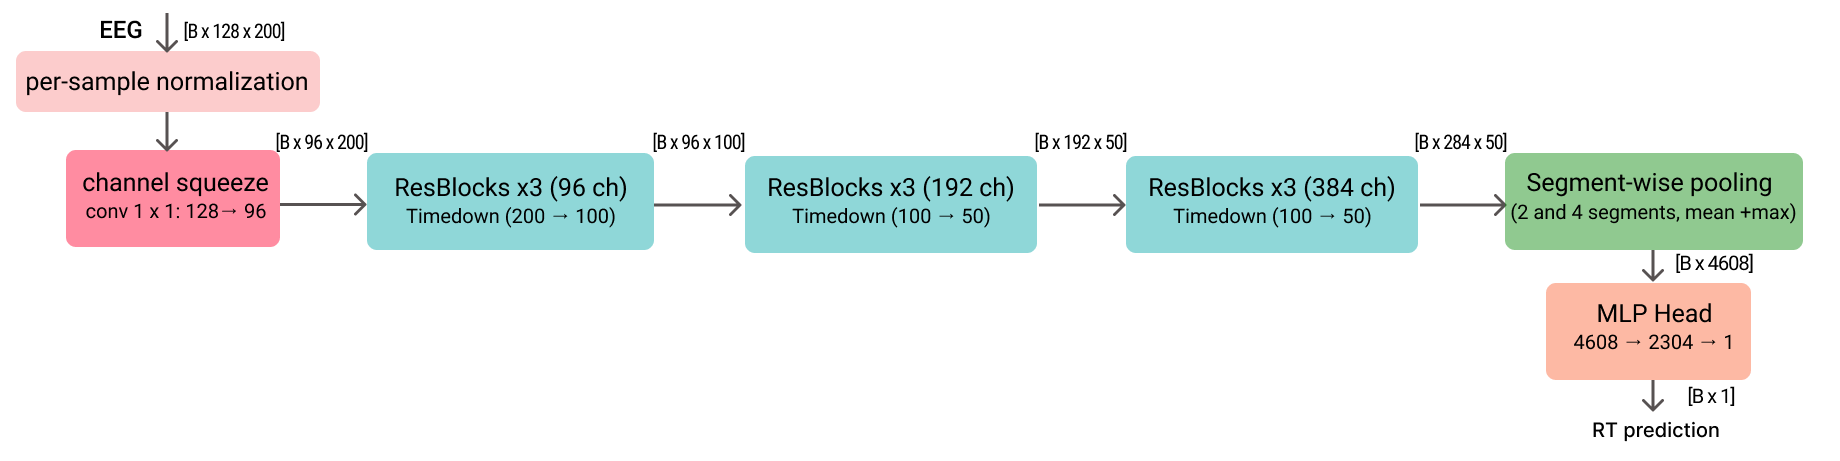
\includegraphics[width=\linewidth]{img/ch1/Ch1_regression.png}
    \caption{SneddyNet: direct RT regression baseline architecture. A lightweight 1-D temporal ConvNet maps a stimulus-locked 2~s EEG crop (128 channels, 100~Hz) to a scalar reaction-time prediction. Per-sample normalization and a learned $1\times1$ channel-squeeze layer (128$\rightarrow$96) are followed by residual depthwise-separable stages with anti-aliased temporal downsampling, segment-wise pooling (2 and 4 segments; mean+max), and an MLP head.}
    \label{fig:ch1_regression}
\end{figure}




\subsection{Direct Regression Baselines: Model Zoo and Takeaways}
\label{sec:rt_reg_zoo}


\begin{table}[!t]
\centering
\caption{Direct Reaction Time baselines (validation). Lower nRMSE is better. \emph{DS} = depthwise-separable.}
\label{tab:rt_regression_models}

\begingroup
\renewcommand{\baselinestretch}{1}\selectfont % prevent global double-spacing from enlarging table
\footnotesize                                % change to \scriptsize if still too tall
\setlength{\tabcolsep}{3pt}
\renewcommand{\arraystretch}{0.95}

% \begin{tabularx}{\linewidth}{@{} l Y l c c @{}}
\begin{tabularx}{\linewidth}{@{} 
p{0.14\linewidth} 
Y 
p{0.10\linewidth} 
c 
p{0.09\linewidth} 
@{}}

\toprule
\textbf{Model} & \textbf{Key design (high-level)} & \textbf{Temporal readout} & \textbf{nRMSE} $\downarrow$ & \textbf{Size (MB)} \\

\midrule
%%%%%%%%%%%%%%%%% old version
SneddyNet-S &
\textbf{Compact DS-residual encoder}\par
Shallow depth and small kernels emphasize local temporal motifs.
Strong temporal compression yields coarse features suited to pooling. &
StatPool + MLP & 0.9299 & 4.95 \\

\addlinespace[0.3em]

SneddyNet-L &
\textbf{Higher-capacity DS-residual encoder}\par
Wider/deeper stack and larger kernels increase temporal context and channel capacity.
Same coarse temporal hierarchy, but with stronger representational power. &
StatPool + MLP & \textbf{0.9152} & 45.66 \\

\addlinespace[0.3em]

SneddyRTNet-Dilated &
\textbf{Dilated DS-residual backbone}\par
Dilations expand receptive field while delaying temporal compression relative to SneddyNet.
Designed to support distributional timing rather than coarse pooling. &
TimeDist soft-argmax & 0.9181 & 49.24 \\

\addlinespace[0.3em]

RecurTiny EEGRT (ACT) &
\textbf{Tied-weight recursive DS core}\par
Iterative refinement with step conditioning; adaptive computation via ACT halting.
Large effective depth at low parameter cost, paired with distributional timing. &
Recur-ACT TimeDist & 0.9179 & 1.67 \\

\bottomrule
\end{tabularx}

\endgroup

\end{table}


Although our final RT solution uses temporal segmentation, we found it important to document strong regression-style
baselines (including scalar and time-distribution readouts) as a reference point and ablation.
Table~\ref{tab:rt_regression_models} summarizes representative regression-style baselines trained and evaluated under the
same validation protocol.

All baselines implement the same high-level pipeline: \emph{(a)} per-sample temporal standardization,
\emph{(b)} a learnable $1{\times}1$ channel-mixing projection ($C \!\rightarrow\! c_0$), and \emph{(c)} a lightweight
depthwise-separable residual convolutional backbone inspired by DS-ResNet style and MobileNet/Xception
\citep{howard2017mobilenets,chollet2017xception}. They differ mostly in how the final temporal feature map is converted into an RT estimate, that is, the \emph{temporal readout}.
In all cases, supervision remains scalar RT (or an RT-derived target) without explicit event-time labels; TimeDist is used only as a readout parameterization, not as event-time supervision.

We consider three temporal readout families. \textbf{StatPool+MLP} (SneddyNet family) applies segmented mean and max
pooling over time to encode coarse early and late cues (conceptually similar to segment-based aggregation in TSN
\citep{wang2016tsn}), followed by an MLP regressor. \textbf{TimeDist soft-argmax} (SneddyRTNet) predicts a distribution
over time bins and reads RT as its expectation via a soft-argmax (coordinate-regression style) readout
\citep{nibali2018dsnt}. \textbf{Recur-ACT TimeDist} (RecurTinyEEGRT) refines the time distribution iteratively using tied
weights with adaptive computation time (ACT) style halting \citep{graves2016act} and FiLM conditioning \citep{perez2018film},
producing a halting-weighted mixture distribution before the same expectation readout. 
SneddyRTNet additionally uses dilated convolutions to expand receptive field while delaying temporal compression relative to SneddyNet \citep{yu2016dilated}.

We observe two patterns emerge. First, increasing capacity improves StatPool+MLP performance
(SneddyNet-L vs.\ SneddyNet-S). Second, time-distribution readouts can match large regressors while being substantially
more parameter-efficient (RecurTinyEEGRT at 1.67\,MB). However, despite being competitive, these direct regression
baselines are less robust under heavy temporal jitter and cropping. Moreover, calibration under cross-subject and cross-release shift is not guaranteed by the readout alone; obtaining well-calibrated uncertainty typically requires additional
modeling and/or post-hoc calibration \citep{guo2017calibration,kendall2017uncertainties}. These considerations motivate the
segmentation formulation below, which makes response timing explicit via event-time supervision and
distribution-matching losses.

\subsection{Reformulating RT Prediction as Temporal Segmentation}
\label{sec:rt_segmentation}

To make event timing explicit and to enable strong crop augmentation, RT prediction was reformulated as
\emph{temporal segmentation}: instead of regressing a scalar directly, we predict a distribution over time bins and read
out RT as its expectation (Figure~\ref{fig:ch1_pipeline}). Compared to distributional readouts used only as a final head, the key difference here is
that supervision is defined in time coordinates and shifted consistently under crop jitter, so augmentation preserves
the event-time target by construction. In practice, this produced a large performance gain and faster, more stable
convergence, while making crop augmentation safer because the supervision explicitly encodes \emph{where} the event occurs.
This is our RT instantiation of explicit temporal structure: behavior is modeled through event timing rather than static
regression.

\begin{figure}[!t]
    \centering
    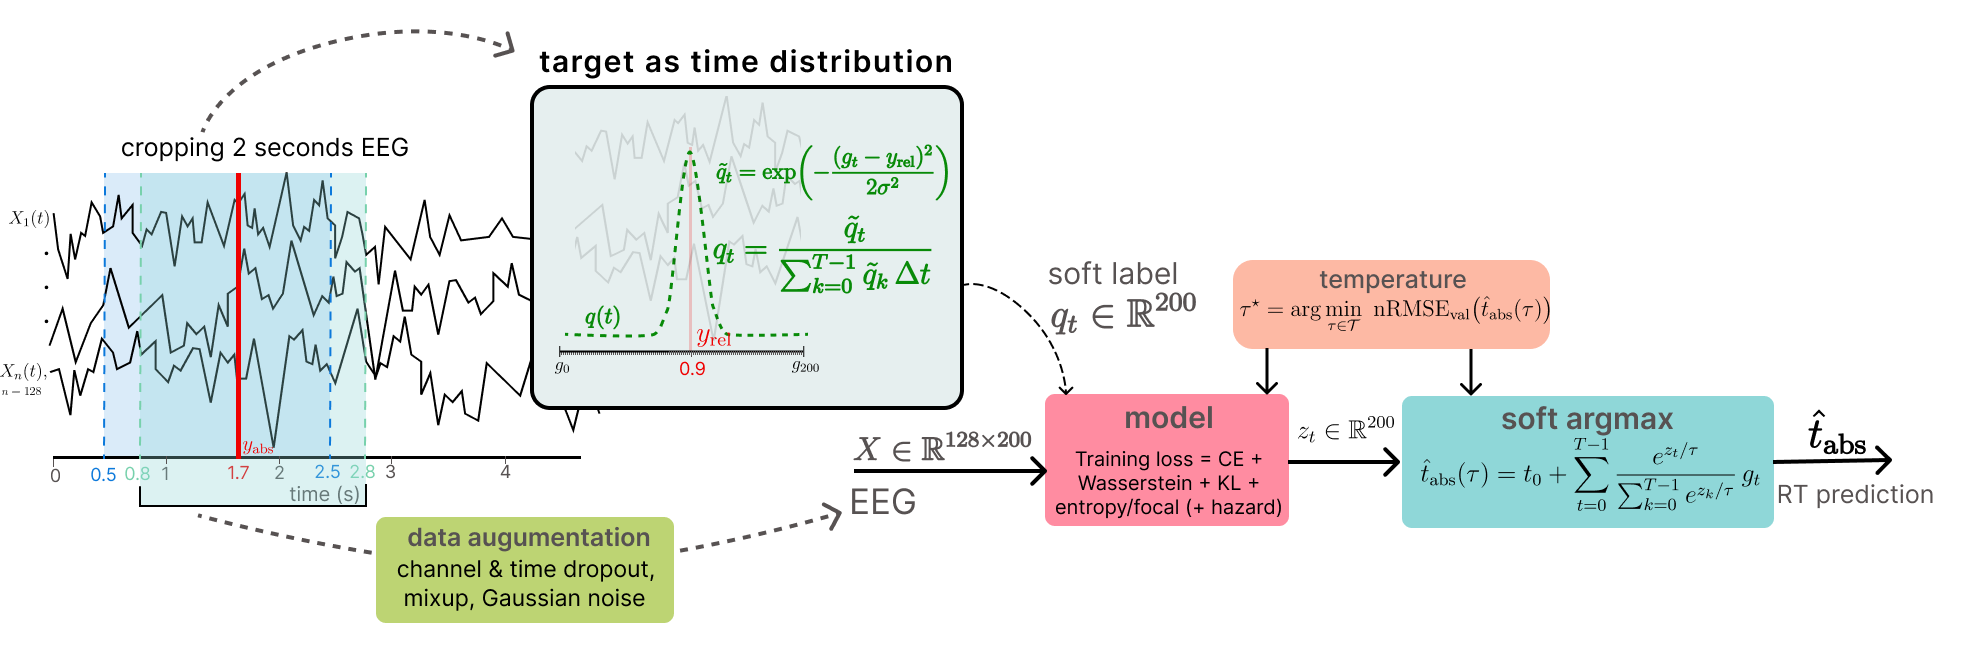
\includegraphics[width=\linewidth]{img/ch1/ch1_pipeline.png}
    \caption{Temporal segmentation pipeline for RT prediction.  For each trial we cache a longer stimulus-locked segment (4~s in our implementation) and sample a 2~s subwindow with start-time jitter for training; the RT label is shifted into the sampled window and a Gaussian soft target $q_t$ is formed. Per-time logits $z_t$ are produced by a 1-D segmentation model and are optimized with distribution-matching losses (e.g., soft-label CE, CDF-based Wasserstein-1, KL, and mild entropy penalty); focal reweighting and a hazard head were explored but not used in the final pipeline. RT is obtained by temperature-scaled soft-argmax, with $\tau^\star$ selected to minimize validation nRMSE.}
    \label{fig:ch1_pipeline}
\end{figure}

\paragraph{Notation and crop sampling.}
Let a 2~s crop be $X \in \mathbb{R}^{C\times T}$ with $\mathrm{sfreq}=100$~Hz, $T=200$ and $\Delta t=1/\mathrm{sfreq}$.
For training-time augmentation, we retain a longer stimulus-locked segment of length 4~s (0--4~s post-stimulus) and sample a 2~s subwindow from it, introducing temporal jitter while preserving trial identity. The crop start is clipped so that the labeled response remains inside the sampled 2~s window (label-preserving jitter). During validation and official inference, we always use the fixed stimulus-locked 2~s window with offset $t_0=0.5$~s (0.5--2.5~s), so that 
$t_{\mathrm{abs}} = t_0 + t_{\mathrm{rel}}$.

\paragraph{Soft target distribution.}
For a sampled crop, the ground-truth event time within the crop is represented as a relative time
$y_{\mathrm{rel}}\in[0,\mathrm{crop\_sec})$ with $\mathrm{crop\_sec}=2$.
A smooth segmentation label is constructed using a Gaussian kernel with bandwidth $\sigma$:
\begin{equation}
\label{eq:rt_soft_target}
\tilde q_t=\exp\left(-\frac{(g_t-y_{\mathrm{rel}})^2}{2\sigma^2}\right),\qquad
q_t=\frac{\tilde q_t}{\sum_{k=0}^{T-1}\tilde q_k},\qquad
\sum_{t=0}^{T-1} q_t=1.
\end{equation}
This smoothing stabilizes optimization while preserving temporal localization; in practice, $\sigma$ can be annealed
(start larger and decrease over training).

\paragraph{Model output and losses.}
A 1-D segmentation backbone (Section~\ref{sec:sneddyunet}) produces logits $z_t$ for $t=0,\dots,T-1$, and a predicted
event-time distribution is obtained via temperature-scaled softmax,
\begin{equation}
\label{eq:rt_pred_dist}
p_t(\tau)=\frac{e^{z_t/\tau}}{\sum_{k=0}^{T-1} e^{z_k/\tau}}.
\end{equation}
Training minimizes a weighted segmentation objective:
\begin{equation}
\label{eq:rt_loss}
\begin{aligned}
\mathcal{L}
&= \lambda_{\text{time}}\,\mathrm{RMSE}\big(\hat t_{\mathrm{rel}}(\tau), y_{\mathrm{rel}}\big)
 + \lambda_{\text{CE}}\,\mathrm{CE}\big(q, p(\tau)\big) \\
&\quad + \lambda_{W1}\,W_1\big(\mathrm{CDF}(q), \mathrm{CDF}(p(\tau))\big)
 + \lambda_{\text{KL}}\,D_{\mathrm{KL}}\big(q\|p(\tau)\big)
 - \lambda_{H}\,H\big(p(\tau)\big),
\end{aligned}
\end{equation}
where  
\begin{equation*}
\mathrm{CE}(q,p)=-\sum_{t=0}^{T-1} q_t \log p_t, \;
D_{\mathrm{KL}}(q\|p)=\sum_{t=0}^{T-1} q_t \log\frac{q_t}{p_t}, \;
H(p)=-\sum_{t=0}^{T-1} p_t \log p_t.
\end{equation*}
The time-RMSE term is the primary objective, since minimizing the readout error aligns directly with the benchmark metric. The remaining terms act as optional distribution-level regularizers on $p(t)$: (i) $\mathrm{CE}(q,p)$ encourages mass near the soft target; (ii) the CDF-based Wasserstein-1 term penalizes temporal
misalignment in a geometry-aware way (shifting probability mass along time rather than matching bins independently); (iii) $D_{\mathrm{KL}}(q\|p)$ discourages off-target modes by penalizing probability mass far from $q$; and
(iv) the entropy penalty $-H(p)$ encourages sharper (more confident) predictions when distributions become overly diffuse under strong
augmentation. We also explored focal reweighting and a hazard-parameterized head (mapping logits to a discrete-time hazard
and then to an event-time distribution), but these variants did not yield consistent validation improvements under the
subject-disjoint protocol and are not used in the final pipeline. We treat augmentation strength jointly with temperature calibration because it affects predictive confidence.

\paragraph{Inference and temperature tuning.}
The relative event time is estimated by expectation (soft-argmax),
\begin{equation}
\label{eq:rt_soft_argmax}
\hat t_{\mathrm{rel}}(\tau)=\sum_{t=0}^{T-1} p_t(\tau)\, g_t,
\qquad
\hat t_{\mathrm{abs}}(\tau)=t_0+\hat t_{\mathrm{rel}}(\tau),
\end{equation}
where $g_t=t\,\Delta t$ denotes the discrete time grid. Under squared error, the Bayes-optimal point estimate is the
conditional mean; accordingly, reading out RT by $\mathbb{E}_{p(t)}[g]$ aligns naturally with the nRMSE objective (RMSE
up to a constant normalization).

In practice, different training choices (loss weighting, augmentation strength, and checkpoint selection) produced
time-distributions with markedly different sharpness and entropy: some models generated very peaked $p(t)$ while others
were systematically more diffuse. This creates a confidence-scale mismatch, where naive averaging (or stacking without
temperature-scaled inputs) can underweight accurate but underconfident models and overweight overconfident ones.

We therefore apply temperature scaling \citep{guo2017calibration} to tune the softness of $p(t)$, improving single-model
readout and making confidence profiles more comparable across models, which in turn stabilizes ensembling and stacking.
Temperature is selected by validation tuning for each base model $m$:

\begin{equation}
\label{eq:rt_tau_tuning}
\tau_m^\star = \arg\min_{\tau\in\mathcal{T}_{\text{cal}}}
\ \mathrm{nRMSE}_{\text{val}}\big(\hat t_{\mathrm{abs}}^{(m)}(\tau)\big).
\end{equation}

In our implementation, $\mathcal{T}_{\text{cal}}$ is a 30-point linear grid in $[0.4,1.8]$ (Table~\ref{tab:ch1_repro}, Sec.~\ref{sec:repro}).

Because confidence scales differ across architectures and augmentation settings, this step is critical; mixup in
particular tends to increase entropy and shift the optimal $\tau$.



\subsection{Segmentation Architecture: SneddyUNet Family}
\label{sec:sneddyunet}

\begin{figure}[t]
    \centering
    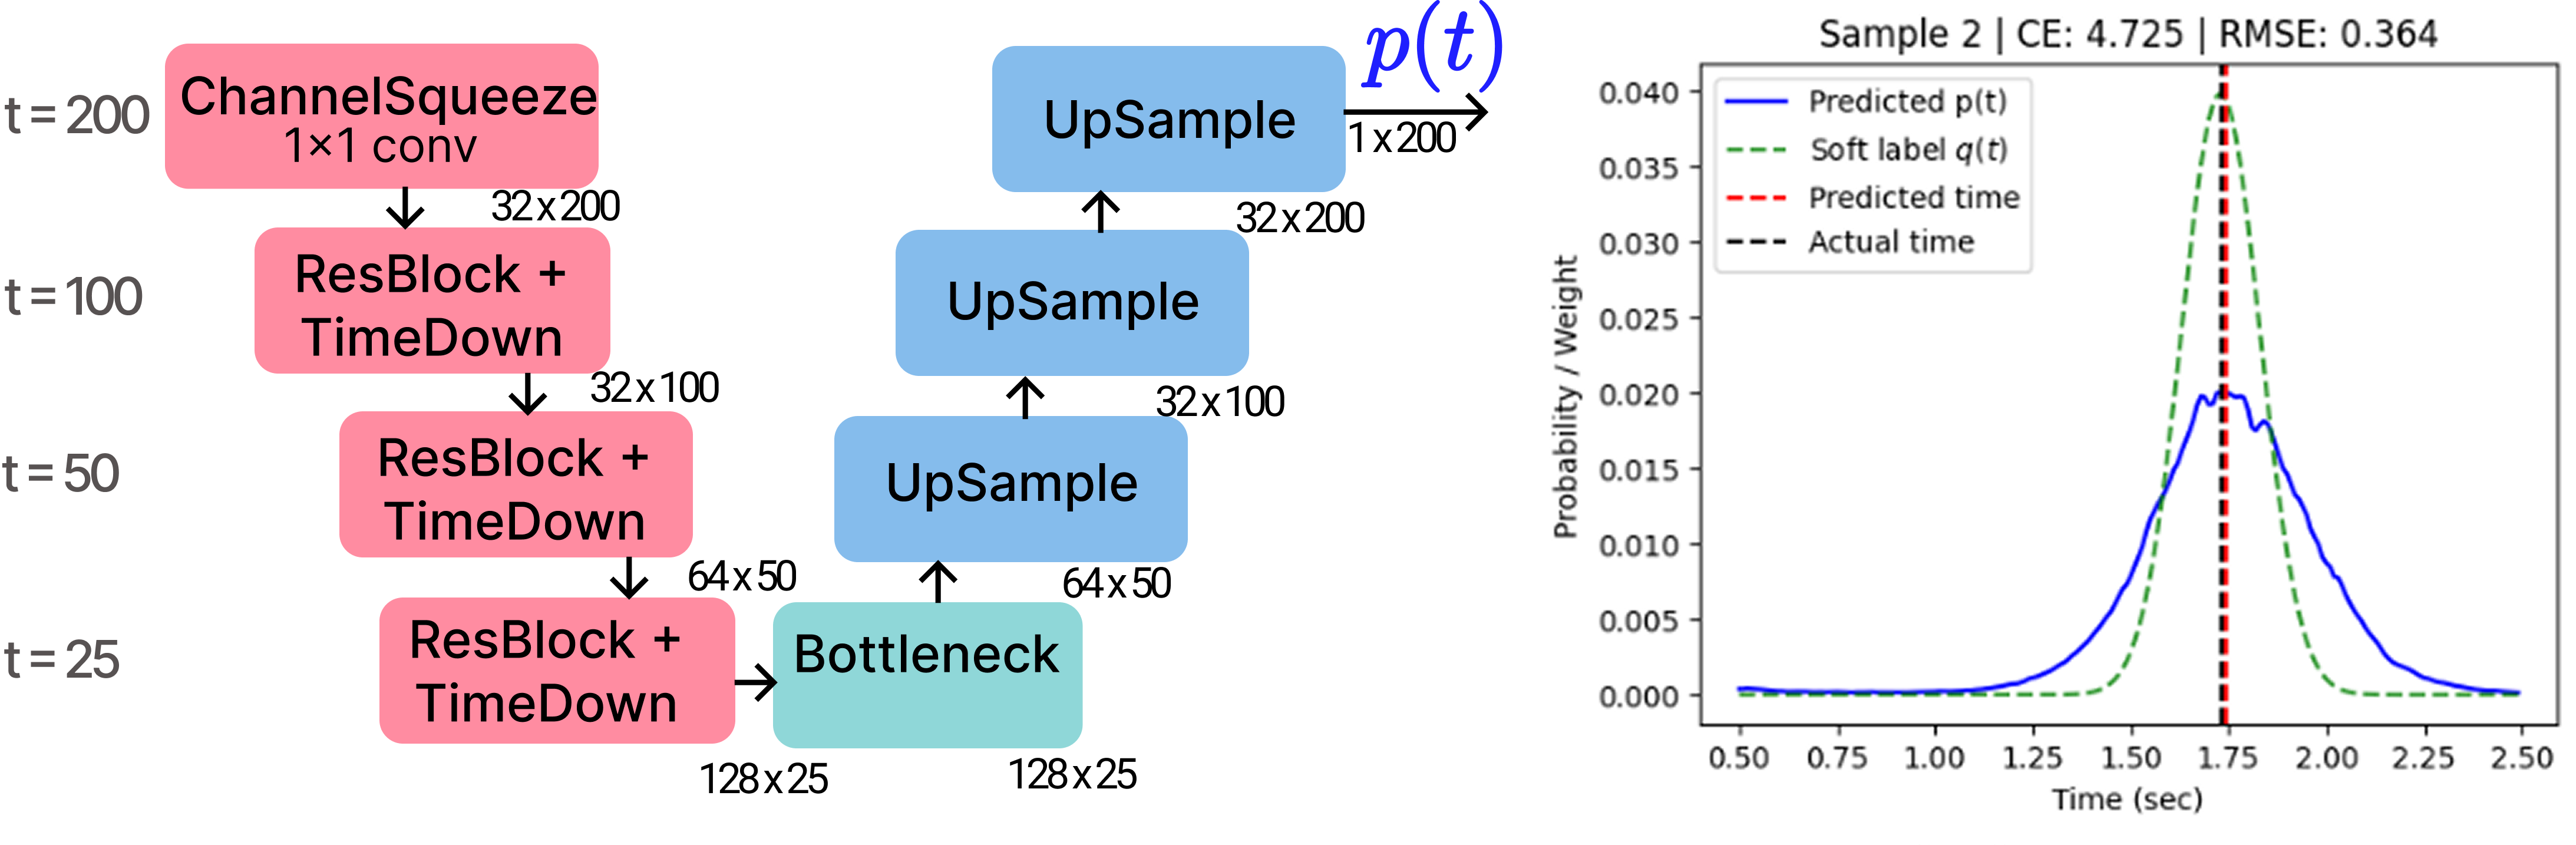
\includegraphics[width=0.9\linewidth]{img/ch1/Ch1_sneddyunet_1.png}
    \caption{SneddyUNet1D for RT segmentation. A lightweight 1-D U-Net maps a 2~s, 128-channel EEG crop to per-time logits
    and an event-time distribution $p(t)$. The encoder applies a $1\times1$ channel-squeeze layer followed by residual
    blocks with temporal downsampling (\texttt{TimeDown}); a bottleneck aggregates context, and the decoder upsamples with
    skip connections to recover time-resolved outputs. The right panel shows an example prediction $p(t)$ and Gaussian soft
    target $q(t)$, together with the resulting predicted vs.\ true response time.}
    \label{fig:sneddyunet}
\end{figure}


A family of efficient 1-D encoder-decoder networks (``SneddyUNet'') is used to map a stimulus-locked EEG crop
$X\in\mathbb{R}^{C\times T}$ to per-time logits $z_{0:T-1}$ (Figure~\ref{fig:sneddyunet}). All segmentation variants follow a 1-D U-Net style encoder-decoder with skip
connections for precise localization \citep{ronneberger2015unet}. The encoder progressively downsamples the temporal axis
to build multi-scale context, while the decoder upsamples and fuses encoder features to recover per-time outputs at the
original 200-sample resolution (internal down/up-sampling is used only to form multi-scale features). Each scale is refined
with lightweight residual blocks (ResNet-style skips) \citep{he2016resnet} built from depthwise-separable 1-D convolutions
for computational efficiency \citep{howard2017mobilenets,chollet2017xception}. To mitigate aliasing under temporal
decimation, downsampling applies a fixed depthwise smoothing filter followed by strided averaging (``blur-pool'' style)
\citep{zhang2019shiftinvariant}. A dilated bottleneck further enlarges the receptive field without additional downsampling
\citep{yu2016dilated}.



\textbf{Segmentation model zoo.} Table~\ref{tab:rt_seg_models} lists the variants used for ensembling/stacking.
SneddyUNet-L/M/S share the same SneddyUNet1D template and vary width and the number of residual refinement blocks per level.
AttnSneddyUNet replaces the bottleneck with temporal multi-head self-attention (MHSA) \citep{vaswani2017attention} and uses
stochastic depth (DropPath) regularization \citep{huang2016stochasticdepth} to stabilize training at higher capacity.
EEGInceptionSeg replaces single-path temporal filtering with Inception-style multi-branch temporal kernels
\citep{szegedy2015going}, following the EEG-Inception design for ERP feature extraction \citep{santamaria2020eeginception}.
Finally, SneddyUNet-FM augments the channel-mixing front-end with factorized cross-channel interactions inspired by
Factorization Machines (FM) \citep{rendle2010fm}, optionally also injected within encoder stages to introduce a distinct
cross-channel inductive bias.


\begin{table}[t!]
\caption{Segmentation model variants used for reaction-time prediction. Each model outputs per-time logits and is trained under the same segmentation objective; architectural diversity is exploited for ensembling/stacking.}
\label{tab:rt_seg_models}
\small
\centering
\renewcommand{\arraystretch}{1.2}
\setlength{\tabcolsep}{4pt} % tighter column padding -> prevents overlap

% Make last two columns auto-wrap to fit the line
\begin{tabularx}{\linewidth}{@{}
  >{\RaggedRight\arraybackslash}p{0.20\linewidth}
  >{\RaggedRight\arraybackslash}p{0.16\linewidth}
  >{\RaggedRight\arraybackslash}X
  >{\RaggedRight\arraybackslash}X
@{}}
\hline
\textbf{Model} & \textbf{Architecture} & \textbf{Key features} & \textbf{Strengths} \\
\hline

SneddyUNet-L (wide)
& SneddyUNet1D
& wider encoder; depthwise-separable convs; 5 ResBlocks/level; dilated bottleneck
& highest capacity; captures complex local temporal patterns \\

SneddyUNet-M
& SneddyUNet1D
& moderate width; depthwise-separable convs; 5 ResBlocks/level; dilated bottleneck
& best single-model accuracy / efficiency tradeoff \\

SneddyUNet-S
& SneddyUNet1D
& lighter encoder; depthwise-separable convs; 3 ResBlocks/level; same bottleneck family
& fast, low-variance; complements deeper models \\

AttnSneddyUNet (MHSA)
& Attention U-Net
& MHSA bottleneck (4 heads, depth=3); DropPath; positional depthwise conv
& captures long-range temporal dependencies \\

EEGInceptionSeg
& EEG-Inception 1D
& multi-branch temporal scales (0.5/0.25/0.125\,s) with feature fusion
& strong multi-scale feature extraction \\

SneddyUNet-FM
& Factorized U-Net
& FM-style cross-channel interactions at input; optional per-stage FM injection
& distinct cross-channel inductive bias \\
\hline
\end{tabularx}
\end{table}





Architectural diversity is introduced to improve ensembling and stacking. SneddyUNet-L (wide) uses a wider encoder and
5 residual blocks per level, providing the highest capacity. SneddyUNet-M retains the same depth (5 blocks/level) with a
more moderate width for a stronger accuracy--efficiency trade-off, while SneddyUNet-S uses a lighter encoder
(3 blocks/level) and yields faster, lower-variance base learners. Long-range temporal interactions are emphasized in
AttnSneddyUNet (MHSA) via a multi-head self-attention bottleneck. EEGInceptionSeg replaces single-path temporal filtering
with multi-branch kernels for multi-scale feature extraction. Finally, SneddyUNet-FM augments the standard channel-mixing
front-end with an FM-style factorized interaction module (optionally also injected within encoder stages), providing a
distinct cross-channel inductive bias.

\subsection{Out-of-Fold Stacking over Time Distributions}
\label{sec:rt_stacking}
Segmentation-style outputs enable richer ensembling than scalar averaging, but combination becomes sensitive to model confidence: naive averaging can overweight overconfident models and underweight accurate but underconfident ones. We therefore train a second-stage stacker on distributional meta-features extracted from the time-distribution outputs.

All base segmentation models are trained once on the training partition $\mathcal{D}_{\text{train}}$
(Table~\ref{tab:protocol}, Sec.~\ref{sec:behavioral_decoding_RT}). We then compute their logits on the held-out validation partition $\mathcal{D}_{\text{val}}$
and convert logits to meta-features (e.g., peak time, entropy/variance, temperature-conditioned expected times, and CDF
quantiles) to train a second-stage stacker. For server-side inference on $\mathcal{D}_{\text{holdout}}$, we compute the
same meta-features from held-out logits and apply the fold-trained stackers (median-aggregated; Figure~\ref{fig:Ch1_stacking}).


\begin{figure}[t!]
    \centering
    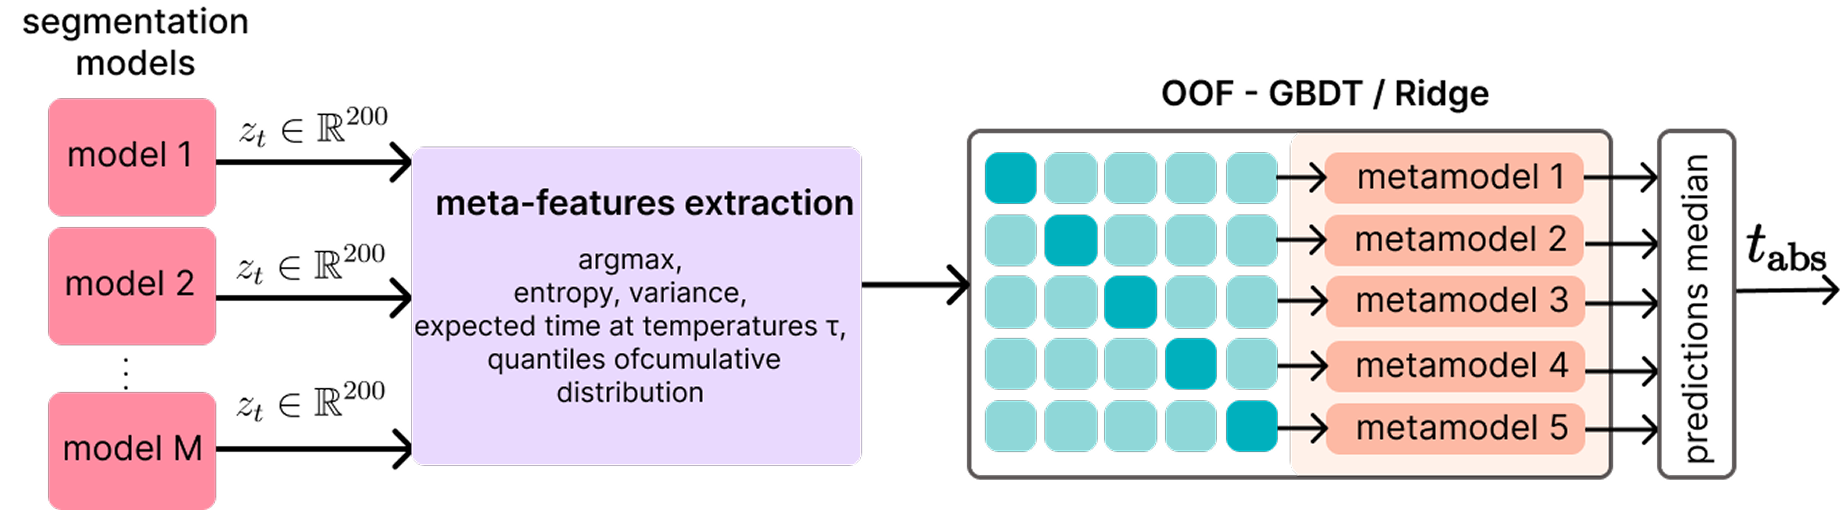
\includegraphics[width=0.9\linewidth]{img/ch1/Ch1_stacking.png}
    \caption{OOF stacking for RT prediction from time-distribution outputs. Per-model logits/distributions are converted into
    meta-features (e.g., peak time, entropy/variance, temperature-conditioned expected times, and CDF quantiles) and combined
    by a second-stage stacker (Ridge/GBDT). Predictions from fold-trained stackers are aggregated at inference (median) to produce the final RT estimate.}
    \label{fig:Ch1_stacking}
\end{figure}

\paragraph{Meta-features from logits and temperature-scaled probabilities.}
Meta-features are extracted per model from (i) raw logits and (ii) temperature-scaled probabilities computed for multiple
temperatures $\tau\in\mathcal{T}_{\text{meta}}$. From logits, a hard-peak estimate and confidence proxies are computed:

\begin{equation}
\label{eq:rt_stacking_logit_features}
t^\star = \arg\max_{t} z_t,\qquad
\hat t_{\mathrm{hard}} = t_0 + g_{t^\star},\qquad
z_{\max} = \max_t z_t,\qquad
m_{\mathrm{top2}} = z_{\max} - \max_{t\neq t^\star} z_t.
\end{equation}
For each $\tau\in\mathcal{T}_{\text{meta}}$, probabilities are formed as $p(\tau)=\mathrm{softmax}(\mathbf{z}/\tau)$ (Eq.~\ref{eq:rt_pred_dist}, Sec.~\ref{sec:rt_segmentation}), where $\mathbf{z}=(z_0,\dots,z_{T-1})$ denotes the per-time logit vector for a given model and window. Distributional summaries
are computed, including the soft-argmax time (Eq.~\ref{eq:rt_soft_argmax}, Sec.~\ref{sec:rt_segmentation}), entropy $H(p(\tau))$, peak probability
$p_{\max}(\tau)$, time variance $\mathrm{Var}_{p(\tau)}[g]$, and CDF time-quantiles (10/50/90\%). In our implementation,
$\mathcal{T}_{\text{meta}}=\{0.7,1.0,1.3\}$ (Table~\ref{tab:ch1_repro}, Sec.~\ref{sec:repro}).

\paragraph{Meta-learner and inference.}
We use linear Ridge regression as a strong baseline meta-learner, and gradient boosting to capture non-linear reliability
patterns across models and temperatures. The meta-learner is trained only on $\mathcal{D}_{\text{val}}$ using 5-fold subject-disjoint cross-validation: each subject is assigned to exactly one fold (Figure~\ref{fig:Ch1_stacking}). For fold $k$, the stacker is fit on the other four folds and predicts RT for the held-out fold. We report validation nRMSE using these out-of-fold predictions. Folds are stratified to match the per-subject mean RT distribution across folds. For inference on $\mathcal{D}_{\text{holdout}}$, the same feature construction is applied to held-out logits; predictions from the fold-trained stackers are aggregated (median) to obtain the final RT estimate. 
Manual blending is retained as a reference, but it cannot adapt weights to sample-specific confidence profiles.


\subsection{RT Prediction Results: Base Models and Stacking}
\label{sec:rt_results}

Segmentation models are first evaluated individually with and without temperature tuning. Compared to the best direct
regression baselines (Table~\ref{tab:rt_regression_models}, Sec.~\ref{sec:rt_reg_zoo}, best nRMSE $\approx 0.915$), segmentation yields a clear
improvement even at the single-model level (Table~\ref{tab:base_models}, best temperature-tuned nRMSE $\approx 0.899$).
This is consistent with the view that making event timing explicit is a stronger inductive bias for RT decoding than
scalar regression in this setting. Wider and deeper U-Nets (e.g., SneddyUNet-M) achieve the strongest single-model
accuracy while remaining efficient, whereas smaller models (e.g., SneddyUNet-S and EEGInceptionSeg) provide
complementary, low-variance predictions that are useful for ensembling. Attention bottlenecks can improve long-range
temporal context but come with higher parameter and storage cost.

The performance achieved by each standalone model is presented in Table~\ref{tab:base_models}, which also reports the
serialized checkpoint size. Notably, the strongest single model (\mbox{SneddyUNet-M}) is only 12.5~MB, and several
complementary base learners are below 10~MB (e.g., SneddyUNet-S: 9.2~MB; EEGInceptionSeg: 0.66~MB). This indicates that
competitive RT prediction can be achieved with lightweight architectures, supporting rapid experimentation and
resource-constrained deployment.

\begin{table}[!t]
\centering
\caption{Representative segmentation models for RT prediction (validation). ``def.'' uses $\tau=1$; ``cal.'' uses the
calibrated $\tau^\star$ selected on the validation split.}
\label{tab:base_models}
\small
\setlength{\tabcolsep}{6pt}
\renewcommand{\arraystretch}{1.15}
\begin{tabular}{lcccc}
\hline
\textbf{Model} & \textbf{nRMSE (def.)} $\downarrow$ & \textbf{nRMSE (cal.)} $\downarrow$ & $\boldsymbol{\tau^\star}$ & \textbf{Size (MB)} \\
\hline
SneddyUNet-L (wide)     & 0.9025 & 0.9023 & 1.076 & 20.8 \\
SneddyUNet-M            & 0.8989 & 0.8988 & 1.076 & 12.5 \\
SneddyUNet-S            & 0.9038 & 0.9038 & 1.000 & 9.2 \\
AttnSneddyUNet (MHSA)   & 0.9015 & 0.9015 & 1.028 & 130 \\
EEGInceptionSeg         & 0.9174 & 0.9169 & 1.124 & 0.66 \\
SneddyUNet-FM           & 0.9105 & 0.9093 & 1.221 & 41 \\
\hline
\end{tabular}
\end{table}

Ensembling is performed at two levels. First, manual blending averages temperature-tuned single-model predictions and
yields performance comparable to the best single model. Second, stacking learns how to combine models based on
distributional meta-features (peak location, sharpness, entropy, variance, and CDF quantiles), allowing confidence to be
re-weighted in a sample-dependent manner. In this setting, gradient boosting provides the strongest overall performance.
Table~\ref{tab:stacking} reports results for different combination strategies on the validation split (stackers evaluated
out-of-fold) and on the organizer-held held-out release (labels hidden).


The improvement from stacking is consistent with the intuition that different architectures produce distinct
time-distribution shapes (sharp peaks vs.\ diffuse uncertainty). By conditioning on distributional meta-features, the
stacker learns when each model is reliable and adjusts their contributions accordingly, yielding a more stable final RT
estimate than fixed-weight averaging.

\begin{table}[!t]
\centering
\caption{Ensembling and stacking for RT prediction (validation OOF and hidden held-out release).}
\label{tab:stacking}
\small
\setlength{\tabcolsep}{8pt}
\renewcommand{\arraystretch}{1.15}
\begin{tabular}{lcc}
\hline
\textbf{Method} & \textbf{Valid nRMSE} $\downarrow$ & \textbf{Held-out nRMSE} $\downarrow$ \\
\hline
Best temperature-tuned single model      & 0.898757 & 0.92334 \\
Manual blending                          & 0.899979 & 0.91840 \\
Ridge stacking                           & 0.890430 & 0.91539 \\
Gradient boosting stacking               & \textbf{0.883365} & \textbf{0.91394} \\
\hline
\end{tabular}
\end{table}

In the next section, we apply the same overarching principle, explicit temporal structure, to trait prediction, where
supervision is weaker and informative signals are captured via lagged temporal coupling rather than event timing.



\section{Reproducibility and Code Availability}

\label{sec:repro}

All code (training and inference), notebooks (data preparation, regression/segmentation, calibration, ensembling and
stacking), and pretrained weights are available at \url{https://github.com/sneddy/neurosned}.

\paragraph{Challenge 1 (RT): exact inference reproducibility.}
We release the exact checkpoints for the base RT models and the fitted stacking meta-models used in our final submission.
Running inference with these released artefacts reproduces our submitted RT predictions.

\paragraph{Challenge 1 (RT): training notes.}
Training uses staged fine-tuning with early stopping on validation nRMSE; on plateaus, we reload the best validation
checkpoint and reduce the learning rate (typically by a factor of $0.5$). Because this procedure is adaptive and GPU
training is not perfectly deterministic, retraining can yield small variations; Table~\ref{tab:ch1_repro} summarizes the
default settings used in our released notebooks.


\paragraph{Challenge 2 (externalizing): inference reproducibility.}
We release the final fitted ridge model used for externalizing prediction together with the feature-extraction code and the
selected feature subset. Running inference with these released artefacts reproduces our submitted Challenge~2 predictions.

\paragraph{Challenge 2 (externalizing): training notes.}
The bootstrap-driven add/drop feature selection is stochastic (bootstrap resampling over subjects); re-running selection can
yield small variations in the chosen subset. Our paper specifies the feature construction (lags, per-window standardization,
ridge-stabilized transitions) and the selection criterion, and the released notebooks implement the exact pipeline.

\begin{table}[t!]
\centering
\caption{Minimal reproducibility details for Challenge~1 (RT). These settings summarize the defaults used in our released
training notebooks and stacking code.}
\label{tab:ch1_repro}
\scriptsize
\setlength{\tabcolsep}{6pt}
\renewcommand{\arraystretch}{1.15}
\begin{tabularx}{\linewidth}{@{} p{0.30\linewidth} X @{}}
\toprule
\textbf{Component} & \textbf{Setting} \\
\midrule
Input / preprocessing &
2~s window at 100~Hz, 128 EEG channels (reference excluded). Per-sample temporal standardization in-model. Official
inference window: 0.5--2.5~s post-stimulus. \\

Training crop jitter (segmentation) &
From a cached stimulus-locked 4~s segment (0--4~s post-stimulus), with probability $p_{\text{crop}}{=}0.3$ sample a 2~s
subwindow with start-time jitter around the default 0.5~s offset (uniform jitter $\pm 0.25$~s), clipped so the labeled
event lies within the crop; otherwise use the fixed 0.5--2.5~s crop. \\

Soft target (segmentation) &
Gaussian label smoothing (Eq.~\ref{eq:rt_soft_target}, ~\ref{sec:rt_segmentation}) with $\sigma=0.15$~s. \\

Segmentation objective &
Primary term: RMSE on soft-argmax time (Eq.~\ref{eq:rt_soft_argmax}, Sec.~\ref{sec:rt_segmentation}); auxiliary terms used when beneficial:
soft-label CE, CDF-based Wasserstein-1, KL, and mild entropy penalty; focal weighting and a hazard-parameterized head were explored but did not yield consistent gains and were not used in the final pipeline. \\

EEG augmentations (segmentation) &
Time scaling ($p{=}0.2$, scale 0.8--1.2), channel dropout ($p{=}0.25$, drop fraction sampled uniformly up to a max value; max 0.8 in our implementation), time cutout ($p{=}0.25$, length 10--60 samples), Gaussian noise ($p{=}0.2$, std $\approx 0.01$--0.04), RT-binned mixup
($p{=}0.1$, Beta($\alpha{=}0.4$)). \\

Loss weights (segmentation) &
Released defaults:
$\lambda_{\text{time}}=3$,
$\lambda_{\text{CE}}=1$,
$\lambda_{W1}=10^{-3}$,
$\lambda_{\text{KL}}=0$,
$\lambda_{H}=0$.
During development, auxiliary weights were occasionally adjusted (or disabled) when beneficial for validation nRMSE;
$W_1$ uses a smaller coefficient due to its larger raw scale. \\

Optimization (segmentation) &
Adam with initial LR $10^{-3}$ (typical), early stopping on validation nRMSE; on plateaus, reload best checkpoint and
reduce LR (typically by a factor of $0.5$; staged fine-tuning). Batch size 2000 in the released notebooks. \\

Temperature scaling (calibration) &
$\tau^\star$ chosen by grid search over $\mathcal{T}_{\text{cal}}$: 30 values linearly spaced in $[0.4,1.8]$
(Eq.~\ref{eq:rt_tau_tuning}, Sec.~\ref{sec:rt_segmentation}). \\

Stacking meta-features &
Per-model features from logits and from $p(\tau)$ at $\mathcal{T}_{\text{meta}}=\{0.7,1.0,1.3\}$: hard peak time,
entropy, peak probability/margin, variance, and CDF quantiles (10/50/90\%). \\

Meta-learner &
Ridge regression (alpha grid) and histogram gradient boosting (lr 0.05, max\_iter 2000, early stopping).
5-fold subject-disjoint CV within the validation partition; fold predictions aggregated by median. \\
\bottomrule
\end{tabularx}
\end{table}

\section{Conclusion}
We studied robust EEG decoding under cross-subject and cross-release distribution shift using the EEG Foundation Challenge
benchmark on HBN-EEG CCD recordings. Our central message is that making temporal structure explicit improves robustness
under heterogeneous, low-SNR EEG. We instantiated this principle in two complementary settings: event timing for
behavioral decoding and lagged temporal coupling for trait prediction.

For trial-wise RT prediction we reported strong direct regression baselines as reference
points and found that objective design, temperature scaling and distribution-aware ensembling provided
consistent gains beyond moderate increases in backbone capacity within the tested regime. The obtained results suggest that scalar regression tends to encourage reliance on global window statistics and exploit global texture-like patterns.  Reformulating scalar regression as temporal segmentation by supervising an
event-time distribution better matched the nature of
the problem and enabled time-consistent crop augmentation. Combining several compact 1-D encoder–decoder variants further improved robustness: their diverse uncertainty profiles could be exploited via OOF stacking on simple distributional meta-features. Stacking helps because different architectures produce complementary event-time distributions. Using distributional meta-features, the stacker learns trial-wise reliability and adapts model weights accordingly, outperforming fixed averaging.


For trait prediction lagged dynamics descriptors help under shift because they deliberately compress each window into regularized, low-dimensional summaries of persistence and cross-channel coupling across multiple time scales. Per-window standardization and ridge-stabilized transitions reduce sensitivity to nuisance amplitude differences and short-window estimation noise, yielding a more consistent trait signal than end-to-end window regression in a weak-supervision regime.


Overall, the most reliable improvements arose when the objective and representation exposed what mattered about
the signal, event timing for behavior and lagged coupling for traits, rather than relying on end-to-end scalar prediction
from short windows. In practice, this favors structure-aligned supervision, calibrated distributional outputs, and combination strategies that exploit complementary uncertainty profiles under distribution shift. At the same time, our conclusions are necessarily conditioned on the specific benchmark design and evaluation protocol, and therefore should be read as evidence about robust prediction under this construction rather than as a definitive statement about underlying neural mechanisms. 


In particular, lagged-transition descriptors are best understood as regularized mechanistic summaries of temporal dependence useful for stable decoding, but not equivalent to causal connectivity or directed neural influence. We also can not claim guaranteed transfer to other tasks, montages, preprocessing pipelines, or populations. These considerations motivate extending the present framework with causal representation learning to better characterize the hidden processes that underlie trait prediction and behavioral decoding, and to build adaptive cross-task pipelines that generalize beyond CCD and remain robust across diverse acquisition settings.


\bibliography{references}






% \bibliographystyle{APA}
% \begin{thebibliography}{100}
% \providecommand{\natexlab}[1]{#1}
% \expandafter\ifx\csname urlstyle\endcsname\relax
%   \providecommand{\doi}[1]{doi:\discretionary{}{}{}#1}\else
%   \providecommand{\doi}{doi:\discretionary{}{}{}\begingroup
%   \urlstyle{rm}\Url}\fi

% \bibitem[{LastName(2009)}]{Ref2009}
% LastName, A. (2009).
% \newblock Title for the first reference.
% \newblock \emph{Journal of the first reference}, \emph{3}, 18 -- 88.


% \bibitem[{Authors et~al.(2008)Author1, Author2, \&
%   Author3}]{Ref2008}
% Author1, A., Author2, A., \& Author3, A. (2008).
% \newblock Title for the second reference.
% \newblock \emph{Journal for the second reference}, \emph{5}, 188 -- 200.

% \end{thebibliography}
\end{document}